\documentclass[a4paper]{article}
\usepackage{a4wide}
\usepackage{graphicx}
\usepackage{hyperref}
\begin{document}
\title{Sesame \vspace{10pt} \\
\large The world first KYT aggregator for AML compliance}
\maketitle
\section{Introduction / executive summary}
Blockchain  \\
The future \\
As blockchain and crypto-assets become widely adopted and regulated, 
However, the ecosystem is not secure yet. \\

First of all, by definition, one doesn’t know with whom they’re interacting as this technology is based on cryptography and pseudonymity. On the other hand, regulation is still inadequate and regulatory authorities are becoming wary of money laundering activities and terrorist financing. These still may represent billions of dollars in terms of illicit transactions. \\

Thus, visibility over the source of funds is becoming a crucial issue for regulators as well as for businesses and individuals. A global interest is currently exploding within the industry towards a common understanding for more compliance, transparency, and legality to foster mass adoption and welcome billions of new users. 
To achieve this goal, the analysis of on-chain transactions, the so-called “KYT” or Know Your Transaction,  remains the key element for verifying the origin of transferred funds, the compliance of each and every wallet, and the legality of transactions. \\

More than 95\% of crypto wallets never had any interaction with tainted funds, therefore more than 95\% of the transactions are undisputable. Our goal is to set the remaining ones aside and create a secure and safe economy within a free and privacy-protecting industry. \\

Within this perspective, regulation is being reinforced. Regulators want to keep a tight rein on crypto-businesses, and above all make sure that is not a go-to way for laundering illicit funds from crime, scams, or ransomware. Businesses, NGOs, entrepreneurs, foundations, investors, and each and every social individual likewise work, grow, and make money in an environment that is respectful of human rights and dedicated to the growth of the rest of society.

\subsection{The Company}
Sesame.fi is a French-based leading company specializing in crypto compliance. We aim to build the next global compliance standard for Web3 and accelerate its adoption by regulated entities and individuals with transparency needs. \\

The crucial part that we are going to implement in the AML process is the Know You Transaction (KYT) procedure. It aims to evaluate financial transactions for fraudulent or suspicious activity. \\

With high-standard compliance AML providing partners, Web3 teams of experts, and Web3 products partnerships, we are ready to achieve one of the most awaited needs in terms of transparency in the industry.

\subsection{Core Team}
As a French-based fintech startup, we gathered a team of solid and complementary experts to join forces in various domains and industries, all involved in Web3 and Blockchain for many years, to succeed in this new entrepreneurial journey: 

\begin{itemize}
\item Christophe Ramananjaona

PhD geophysicist and high-performance computing developer with more than 20 years of expertise gathered around the globe in data processing and numerical models for academia and the oil and gas industry with a keen interest in smart contracts and leveraging blockchain technology;

\item Cyril Chadé

Serial entrepreneur, investor and government advisor created 4 companies in web 1, web 2 and web 3, successfully exited 2 of them. Advisor to European governments, ministers, law-makers, and institutions. Advisor of numerous tech companies: Google, Facebook, Lime;

\item Roger Krondorf 

Founder of 3 companies, creative director and UX expert (Mercedes, Microsoft).
\end{itemize}

\subsection{The issues}
As blockchain and digital assets become more widely adopted and regulated, banks and financial institutions, as well as luxury brands, artists, auctions, real estate, medical researchers, logisticians, and many more want to enter the decentralized world with as much guarantee as possible to:

\begin{itemize}
\item Buy and Sell digital assets
\item Fulfill the needs of their customers
\item Take advantage of some decentralized finance products
\item Build their own services and applications in a distributed ledger
\item Inter-operate using a more secure, transparent and efficient technology
\end{itemize}

All these actors are more and more vigilant concerning the way the market is behaving. Our industry is pressured by international competition, but also willing to adopt common standards to allow mass adoption. Compliance standards are being approved as they are being created and enforced, in order to provide healthy conditions for economic growth in the blockchain space. \\

Customers who want to enjoy decentralized products and services, and wish to take part in this revolution, deserve compliant ecosystems. \\

Individuals use Web3 products (DEXs, NFT marketplaces, etc) without knowing the counterparty they are dealing with. In a decentralized exchange as well as on NFT marketplaces the origin of funds is absolutely unknown. Pseudonymity is one of the beauties of Web3, and though identities and privacy must be protected, transactions can, and should, be entirely traceable and tracked. \\

This current structure of the market deters large financial actors and other compliant bodies like non-profit organizations from participating in this industry. Billions of dollars are thus missing in the ecosystem, due to a lack of guarantees and compliance. \\

In short, individuals, financial institutions, companies, NGOs and states are all facing the same issue: 

{\it How do we clearly identify malicious actors inside Web3 products and put them aside? \\

What kind of mechanism can we set up to create a risk-less space for legit actors?} \\

This is how Sesame.fi addresses these questions.


\subsection{The solution}
Sesame.fi aims at giving the keys to accelerate crypto adoption by providing maximum transparency for all of its users. Anyone, whether it is an individual, a business, a builder, an investor, a bank, or a crypto project, can check any wallet of her own, track its transaction history and make sure it has never dealt with illicit activities. \\

By creating Certified Web3 Spaces\texttrademark\ in real-time with a global “whitelist” of positively scored addresses, and checking those with which they are interacting, we can open new possibilities for the Web3 space, and create a secure environment. \\

As a direct answer to regulatory pressure that is coming right now, our standard of compliance is higher than the actual world-class banking standard. Being associated with four AML providers to date, and more to come, we provide the most accurate compliance tool in the whole industry. \\

Through our mastery of decentralized technologies, we provide a certification that will guarantee, in real-time, that millions of blockchain participants can transact without worrying about the risk associated with the origin of funds of their counterparty. \\

Our solution will create a flood of trillions of dollars from worldwide institutions and skeptical individuals who have been waiting for more compliance before tipping their toes into the blockchain space.

\subsection{Advisors}
We strongly believe in collective strength, mutual learning and team synergies. Blockchain and crypto technologies are based on math before being an ecosystem, and finally a business. We have surrounded ourselves with people with the highest theoretical and practical experience in the blockchain industry to build and deploy these new tools and services, from a compliance standard to safe spaces and on-chain certifications. \\

As part of our development, we rely on experts to share ideas, and improve on the latest discoveries and technologies which can provide the answers we need. This is why we will have experts with different profiles in order to build a complementary group. \\

With this in mind, we have created 3 groups of experts: 

\begin{enumerate}
\item The first one focused on compliance, legal, governmental relations, public affairs and regulations on an international scale. 
The purpose of the first group is to accompany us on the legal part in connection with Web 3, its ecosystem, and the current changing regulations. This strength will allow us to have a product tailored to current standards.

\item The second group focused on research, and technology, coming from world-class universities and laboratories. These experts will provide us with technical support in building and implementing the certification.

\item Last but not least, we will benefit from the help, vision, and knowledge of tier-one entrepreneurs and business leaders, creating opportunities, and challenging our goals and vision.
\end{enumerate}

Thanks to this tailor-made support, our compliance standard is ready to become the universal certification that the ecosystem needs.

\subsection{Partners}
Sesame works with key players, movers, and shakers of the digital asset ecosystems, in particular anti-money laundering (AML) providers, to provide regulated entities with a single query that will aggregate and verify the data from a client wallet using all the providers available, hence reducing operational and compliance risk associated with using only one provider.


\subsubsection{AML Providers}
We have been selecting four key players in the ecosystem and we are happy to have reached a collaboration agreement with them. 

\begin{itemize}
\item Merkle Science

Founded in 2018, Merkle Science is a predictive cryptocurrency risk and intelligence platform that helps entities detect, investigate, and prevent illegal activities involving cryptocurrencies.


\item Crystal

Crystal powers cryptocurrency transaction analysis and monitoring on the blockchain, bringing best-in-class AML compliance and risk management solutions.


\item Blockchain Intelligence Group (BIG)

Blockchain Intelligence Group builds technology to power compliance and intelligence for the blockchain-centric future


\item Scorechain

Scorechain Analytics tracks crypto assets and helps create a structured and coherent approach to identifying, assessing and managing risk. 


\item Chainalysis

\end{itemize}


\subsubsection{Investors}
We aim to look for investors who are going to be our ambassadors. At the same time, we could have the ambition that these partners concerned by KYC-AML-KYT issues will also be motivated to support us. 


\subsubsection{Law firms and Compliance Officer}
Compliance Officers became a key element of any worthy crypto company. On the external side of compliance, law firms always play a crucial role in helping nascent technologies keep up with the regulatory updates. Both those actors are natural partners and prescriptions for Sesame.

\section{SESAME: The first-ever crypto compliance certificate}
\subsection{Introduction}
We are proud to introduce the Sesame Certificate: the digital compliance certificate used to create Certified Web3 Space\texttrademark\ in Web3. \\

By doing KYT in real-time checking of any address and being an owner of a Sesame Cetificate, we guarantee our users access to whole new compliant spaces in the industry such as DeFi, NFT Marketplace, Metaverse, or any Web3 products.

\subsection{SESAME v1.0}
Our simple interface gives any user the possibility to obtain a certificate in less than 2 minutes. In the back-end, we perform a query to all of our AML providers in order to verify the legitimacy of the address, and by the aggregation of all scores into our tool we can assess if an address interacted with funds related to financial crimes with higher certainty. \\

This service is accessible to anyone and scoring an address only costs \$3. All the blockchain interactions from the Sesame solution go through the Avalanche blockchain to minimize cost for the end-user. Thanks to our technology stack, the user can score any compatible address and pay from any blockchain while we handle all the whitelist operations from the Avalanche blockchain. \\

After validation, the address will immediately be whitelisted in our smart contract. The presence of an address in the whitelist smart contract has the validity of a certificate. This certificate works as a passport and represents the analysis that funds do not seem subject to illicit activities. This certification will be valid for a limited period of time (90 days) and will require renewal after this period. Conversely, a user staking a defined amount of Sesame tokens could benefit from the service as long as the tokens remain staked in the staking smart contract. \\

Furthermore, a monitoring service checks in real-time the score associated with counterparty addresses whenever it transacts with a whitelisted one on the blockchain and updates the whitelist according to the scoring result of the counterparty, block after block. \\

Every time a transaction involves a whitelisted address, our monitoring tool detects it and automatically renews the scoring to check if the address is still allowed to be in the whitelist by either having transacted with another whitelisted address or with an address with a compliant score. If not, the address is removed from the whitelist.
The tool will work for all the blockchain tokens monitored by the AML providers. \\

By leveraging on-chain smart contract technologies, we can guarantee the transparency of the system and the compliance of all the addresses. Thanks to our partnerships with the leading AML providers we can obtain the resiliency and the most accurate scoring in the world.

\subsection{Multi-Chain compatibility}
Leveraging the technology of our AML providers, we can explore and create a compliant safe space for more than 25 blockchains. We plan to first invest in the Ethereum blockchain, where most AML providers offer compliance analyses, then we will look into the other EVM-compatible blockchains, like Tron, Binance Smart chain, Ethereum Classic, Avalanche, layer 2 chains, before opening our tool to non-EVM compatible blockchains (Bitcoin, Cardano, Solana, Algorand, …). For more details about Sesame deployment see the roadmap section. 

\subsection{Building a universal standard}
Blockchain has unique characteristics that make it so interesting: its pseudonymous, transparent, decentralized, and secured consensus. \\

Those characteristics brought tremendous innovation but also had minor drawbacks.  The rise of cryptocurrencies was quickly followed by the birth of a thriving black market ecosystem on the web, capitalizing on the strength of blockchain technologies. Even though law enforcement has stopped the vast majority of those activities, a significant portion of crypto transactions is used to launder proceeds from real-world criminal activities. Lastly, with the advent of DeFi, hackers have been relentlessly abusing the flaws in the protocol setups and codes to steal millions of dollars. \\

Sesame’s intention is to create Safe Spaces through Web3, to marginalize bad actors and tame crypto assets. In time, our Certified Web3 Spaces\texttrademark\ will grow as more and more users and projects will comply with the nascent crypto regulations. In the end, a vast majority of crypto markets will become safe spaces filled with lawful users and legit transactions. \\

Sesame will capitalize on the strength of blockchain technology to create a universal standard for KYT and a fully transparent, pseudonymous, and secure passport to enter those Certified Web3 Spaces\texttrademark, the same way malicious actors have profited from it. \\

This standard will be built by setting parameters from AML providers which best represent the international standard of financial compliance and aggregate the results.

\subsection{Certified Web3 Space\texttrademark\ licensing}
During the first stage of the project, Web3 projects will be able to use our Certified Web3 Space\texttrademark\ label at no cost, given that they fulfill the best practice requirements of the Certified Web3 Space\texttrademark\ specifications. Any Web3 project dealing with crypto-assets can claim the Certified Web3 Space\texttrademark\ label. \\

In a second stage, the Certified Web3 Space\texttrademark\ gateway can allow tailor-made filtering of the users depending on their requirements and jurisdiction. * geographical/legal framework settings* Partners wishing to opt for this kind of solution will be able to get support from Sesame to define the settings of the AML score aggregation and will de facto use a specific whitelist, representative of their affiliated jurisdiction (i.e. ban on gambling-related tokens in Korea, upcoming MiCa regulation in Europe, etc.). \\

Lastly, the Certified Web3 Space\texttrademark will need to bring some advantages to the users taking the compliant way. Those advantages might be materialized as priority access to new services or advanced features that are easier to launch for a compliant crowd, extra basis points on the stacking and yielding rewards, or even only allowing Sesame-certified users the access to specific services like an auction, a marketplace, etc. The idea is simple: compliance should be rewarded. 

\subsection{Additional revenue streams}
\subsubsection{Bridging the gap between Web3 and compliance}
Developers of Web3 products can attract new sources of funds, especially from institutions and individuals with a need for compliance. Moreover, the pressure from regulators is higher than ever before and incentivizes all Web3 actors to start looking for a way to reduce the compliance risk associated with criminal activities. \\

We are also offering a Legal Consultancy Service (additionally to our technical product) that can advise any Web3 owner on the latest rules in terms of crypto compliance and the way how they can fulfill the requirements enforced by law, depending on the jurisdictions where they have established their activities. This will bring an educational aspect to the web3 actors and will be possible thanks to our advisors. A team of technical sales will be available to help them integrate the Certified Web3 Space\texttrademark\ into their products for future customers. \\

By partnering up with more and more law firms and law professionals, we aim to integrate our Certified Web3 Space\texttrademark\ into all Web3 projects to help them reduce the regulatory risks.

\subsubsection{Premium services}
From small fishes to shrimp sharks and whales, everyone will be given the opportunity to score their various wallet addresses at a fixed price. When a scored wallet comes out with a significant amount of crypto, the owner will have access to a different user experience and an opportunity to subscribe to extra services designed to cater to his specific needs. \\

For this type of high-value wallet, we offer a range of compliance and intermediary services for a fee of 0.1\% of the value of the wallet. 

\subsubsection{Institutional Scoring}
Sesame aims to create a safer and more compliant Web3 at minimal cost for the public but is also able to adapt its solution to the needs of financial institutions. \\

For instance, a wealth manager launching a new crypto service for its client base could benefit from our scoring capacities to make sure his client's funds are compliant with his jurisdiction regulation, before accepting to manage their crypto assets. \\

Then, each time new clients want to enter the service or add new crypto funds to their portfolio under management a scoring can happen. For this part of the business, we offer both on-chain and off-chain scoring depending on what our interlocutor is more comfortable with. Of course, everything is handled with the utmost privacy meaning that none of the score addresses can be found.
\section{The Sesame (SAM) token}
\subsection{Utility}
\subsubsection{Utility vs Security Tokens}
A lot of people are not aware of the differences
between utility and security tokens because of
the fact that in a way, they are in the same basket.
The biggest similarity is that both of these tokens
are given out in exchange for capital. However, in
a way, a utility token is like a digital coupon which
can be exchanged for discount on fees, special
access to features or services. On the other hand
a security token is an asset that derives its value
from an external asset but it is also subject to strict
federal law regulations imposed by the state.
The DOPE token falls under the utility tokens
category.[a]


\subsubsection{Claiming a certificate after a successful Scoring}
For individuals who want to access Certified Web3 Space\texttrademark, the registration of the Sesame Certificate is mandatory. In order to claim it, every address that wishes to be registered has to pay through our tool to get a score. These funds will be used to create long-term sustainability for the project. In the long-term, we are aiming to create a DAO and these funds will directly go into the DAO vault in order to finance the project. 

\subsubsection{Staking : access to premium services}
As we mentioned before, after every transaction made by a whitelisted address, the compliance has to be refreshed (except if the transaction occurred with another whitelisted address) in order to verify if the address is still legitimate. Every whitelisted user has to go back to our tool in order to re-score his address and claim the Sesame Certificate again after every transaction with a non-compliant address. Any user that stakes 60 SSM will get lifetime access to scoring and automatic renewal of the certificate for any of his addresses. 

\subsection{Tailor-Made Compliance Certificate} 
Any Web3 product can freely integrate the Certified Web3 Space\texttrademark\ label into their products. Without permission requirements, they can create Certified Web3 Space\texttrademark\ using our open-source repository of smart contract ABI (application binary interface) and start to onboard Sesame Certificate owners on their products. In this case, users will have access to any Certified Web3 Space\texttrademark\ product through their certification recorded in the white list smart contract.


\subsection{Tokenomics}
\subsubsection{Token description}

\begin{itemize}
\item Token ticker: \$SAM
\item contract addresses: ETH 
\item Total Supply: 100 000 000
\item Initial Circulating Supply: 
\item Initial Market Cap on listing: 
\end{itemize}

The Sesame token (SAM) main purpose is to unlock lifetime access to the Sesame KYT solutions. Initially, users will need to stack 60 SAM to get access to our scoring and monitoring service. For stacking users the main upside is they can add funds and interract outside of the Certified Web3 Spaces\texttrademark\ without needing to pay again to make sure their wallet is still compliant. 

\subsubsection{Lock-up and dedications}

\begin{itemize}
\item Private sale Seed: 15\% - Vesting over 24 months after TGE

\item Private sale 2: 10\% - Vesting over 36 months after TGE

\item Launchpad and IDO fund: 3\% - Fully unlocked on TGE

\item Direct listing liquidity fund: 2\% - Fully unlocked on TGE

\item Team allocation: 10\% - Vesting over 24 months after TGE

\item Advisor allocation: 10\% - Vesting over 24 months after TGE

\item Partnership Fund: 10\% - Vesting over 12 months after TGE

\item Strategic reserve: 10\% - Vesting over 12 months after TGE

\item Token sold for stacking: 25\% - Fully unlocked on TGE
\end{itemize}


\subsubsection{Distribution visuals}


  

  





\subsubsection{Executive Token economics}


\section{Customers}
\subsection{Web3 products}
\begin{itemize} 
\item Decentralized Exchanges

Dedicated pools can be very interesting for institutions that want to buy cryptocurrencies for their customers. A Certified Web3 Space\texttrademark\ ETH/USDC pool would be a game-changer for a lot of banks and funds in order to reduce their risks of being used as launderers. Liquidity providers owning the Sesame Certificate on their side could ask for a higher APY by guaranteeing the clean nature of their funds. 

\item Launchpads

Launchpads are facing pressure from regulators due to the volume of funds they handle; several ICOs have been conducted without any KYC or anti-money laundering control. We will create Safe Spaces inside launchpads such as Pancake Swap or Trustpad to allow them to be compliant with regards to anti-money laundering policies. By accepting only Sesame’s whitelisted wallets, these actors will reduce the risk of hosting tainted funds, thus easing the burden of the ever-growing regulatory framework. With Sesame, decentralized finance can comply with the harshest regulations.


\item Wallets

A wallet provider would be happy to help his customers know if an address that they are on-boarded is holding a Sesame Certificate. This will reduce the compliance risk for wallet providers evolving in strict regulatory environments. 

\item Chains

On a wider global scale, we can partner with chains in order to ensure the compliance of all their total value locked. Scanning wallets, and helping new projects to integrate a Certified Web3 Space\texttrademark\ would help project and in-fine the chains to attract a lot of institutions and individual investors.

\item Metaverse

Several high-profile companies are preparing crypto-based online casino and sports betting systems. But both are infamously known for helping to launder money in the real world, so why would it be different in the Metaverse? By introducing Certified Web3 Space\texttrademark\ into Metaverse, we can imagine a new way for people to interact safely. From a compliant crypto casino to a famous brand, we can guarantee any actor that no one will be impacted by criminals' activities. A new advertising angle can also be imagined in these spaces: a real estate company can, in full confidence, advertise on the web page of a Certified Web3 Space\texttrademark\ with confidence that the ads are only targeting compliant users.

\item NFTs Marketplace

Much like casinos, art is known to be a way of laundering dirty profits, and the issue is already creeping up on NFT Marketplaces. With our solution, auction houses and NFT marketplaces can create a gateway to allow only Sesame Certificate holders to participate in a sale, exclude tainted coins and drastically reduce the risk of money laundering; thus creating a safer digital art space furthering art and creativity.
\end{itemize}

\subsection{Financial Institutions and Financial Service Providers}
Nowadays, getting into crypto is a strategic priority for most financial institutions. However, this new financial Far West presents substantial risks. Institutions need reliable partners to get past those and benefit fully from the opportunities offered by crypto. Our tool suite will help any actor with the due diligence process and client monitoring so that she can expand in the crypto space with minimal risk exposure.
Diving into the crypto space after years in a given sector is a significant challenge. However, offering crypto services will become absolutely necessary for all financial institutions in the coming years. By integrating the Sesame KYT solution to its existing KYC and AML procedures any wealth manager or bank will be able to onboard a trove of crypto-holders as clients with minimal risk and an individual scoring for all of their addresses. For the part of the Sesame solution, we offer both on-chain and off-chain scoring depending on what the financial institution we’re dealing with is more comfortable with.

\section{Technical Architecture}
\subsection{Door 1.0 (2022)}

The first release of the solution will include a frontend where a user can pay for its registration into the whitelist, given that its aggregated wallet score from various AML providers satisfies the compliance criterion (score below a defined threshold value).
The whitelist is an on-chain smart contract managed by the contract owner, meaning that only one wallet is authorized to insert or remove addresses into it. An off-chain “whitelist manager” program is in charge of this task on behalf of the registration frontend or the monitoring program (see Fig.~\ref{offchain}). \\

A duplicate copy of the whitelist is stored in an off-chain database in order to keep a backup of the whitelisted addresses. This off-chain database is also serving the requests of the t monitoring service in order to keep the pace of the monitoring program in sync with the creation of new blocks in the chain (the responsiveness of a central database is notably higher than the decentralized smart contract). Regular checks will be carried out to ensure that the database entries are consistent with the whitelist entries in the smart contract. \\
  
\begin{figure}[!h]
\centering
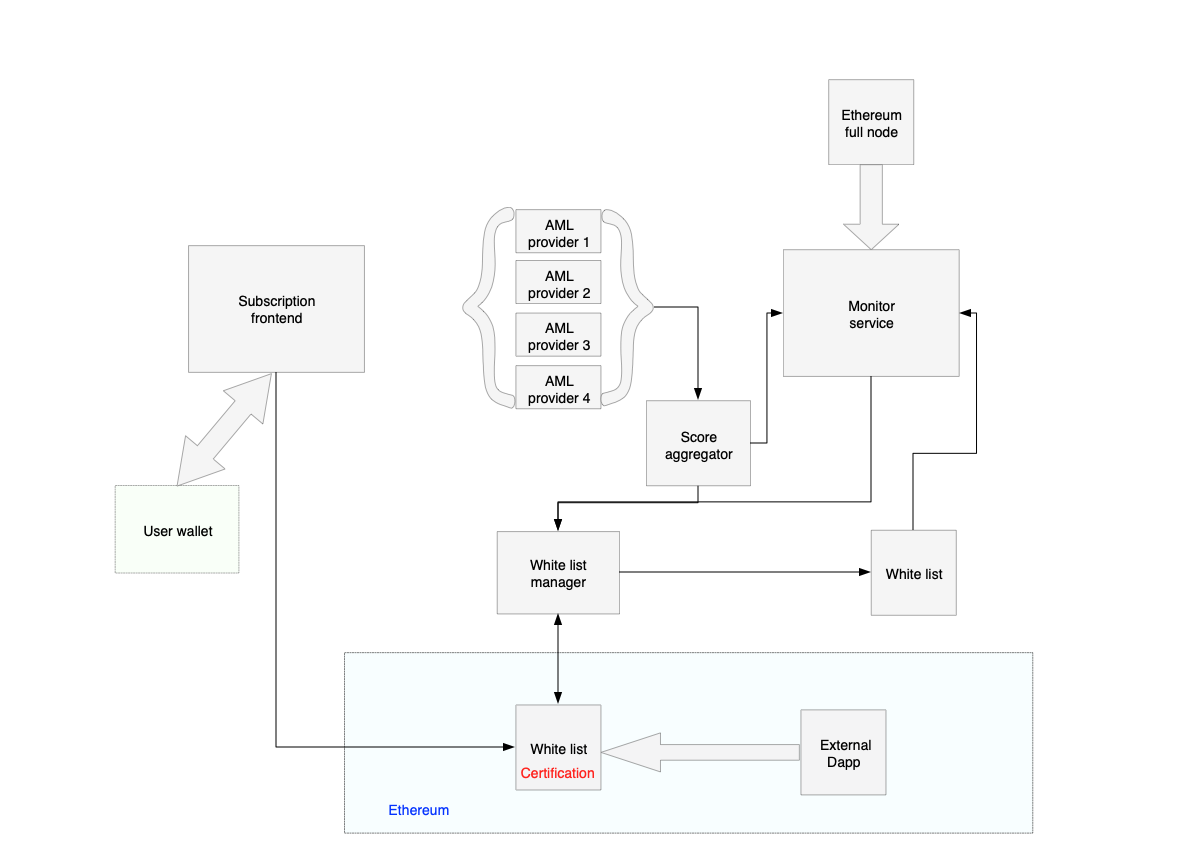
\includegraphics[scale=0.35]{architecture_v1.png}
\caption{Software architecture with off-chain whitelist management}
\label{offchain}
\end{figure}

The monitor program checks every transaction of every block and identifies the addresses which have transferred tokens to the whitelisted addresses. If the counterparty address obtains a compliant score from the AML providers, no change is made to the white list; on the contrary, the monitor program sends a post request to the whitelist manager to remove the recipient address from the whitelist.
Once an address has been registered in the whitelist, an external dapp can call a function of the whitelist smart contract which will return a “true” boolean value to confirm that the address is indeed compliant, and can then authorize this address to transact in the Certified Web3 Space\texttrademark of the Dapp.
For sake of simplicity, the whitelist will be only valid for the blockchain where it has been deployed since decentralized applications will need to make function calls to the whitelist smart contract. However, once the AML providers have aggregated their scores from different EVM-compatible blockchains, meaning that a score will be identical for a given address on every chain where this address holds tokens, it should be technically possible to make function calls to the whitelist on one blockchain and use the compliance result to authorize or prohibit transactions from that particular address on any other blockchain. That solution will remain at the discretion of the decentralized application developer. 

\subsection{Door 2.0 (2023)}

The second version of the solution will make use of an oracle to bring the address scoring comparison with the compliance threshold on-chain and will therefore increase the decentralization and transparency of the whitelisting procedure (see Fig.~\ref{onchain}).
  
\begin{figure}[!h]
\centering
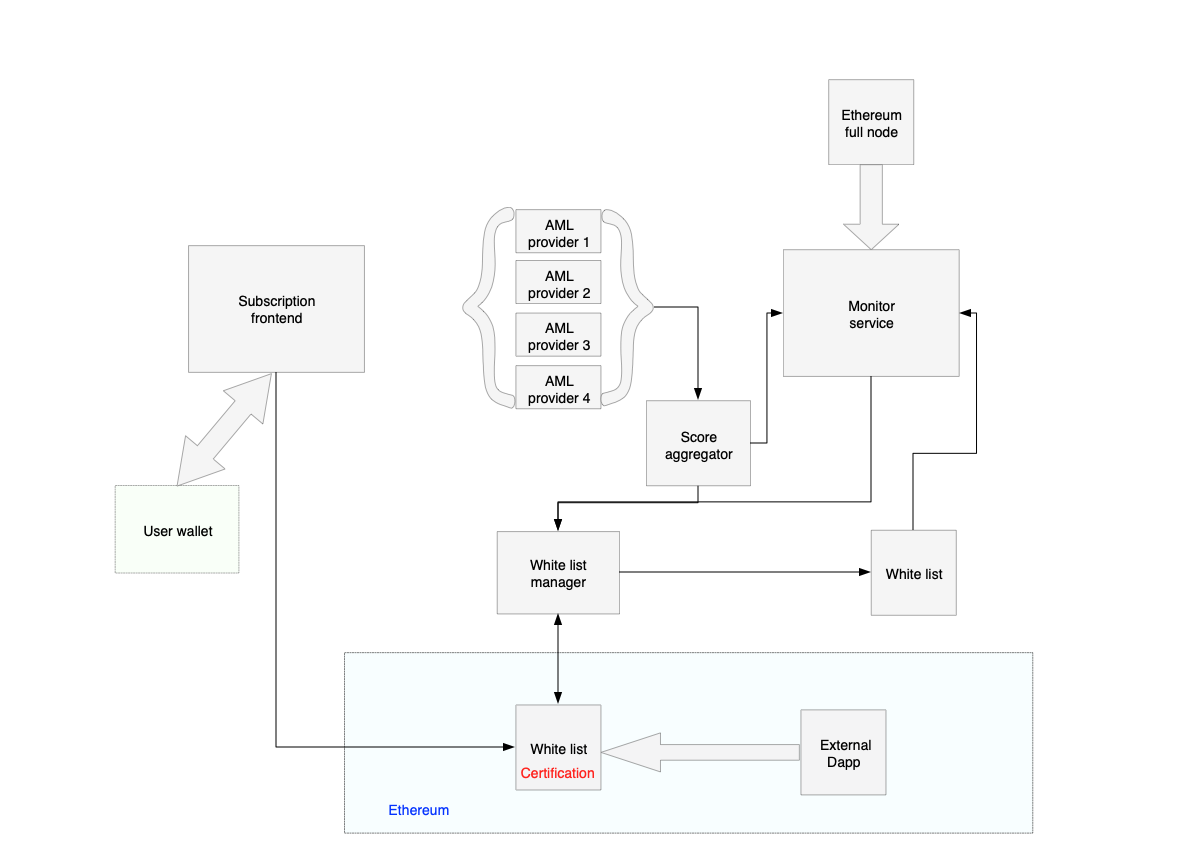
\includegraphics[scale=0.35]{architecture_v1.png}
\caption{Software architecture with on-chain whitelist management and NFT certificate minting}
\label{onchain}
\end{figure}

A separate oracle, and potentially an NFT bridge, could be used to transfer the certificate to another blockchain given that the wallet score for a given wallet has been aggregated by the AML providers.


\subsection{Monitoring service}
The monitoring service can be run directly on an Ethereum full node in order to maximize the processing speed of every transaction, by not making requests through the internet. \\

At some point, the number of transactions in a block might become so large that a single machine might not be able to process all the transactions of the block before the arrival of the next block. In that case, parallel processing based on Apache Spark will so that transaction verification requests can be made to one node or more. \\

In a simplified model where the registration and churn rates are constant, if one also considers the  constant percentage $p$ of wallets transacting every day amongst a total number of wallets $\omega$ , the percentage of wallets registered in the whitelist is given by:
  
$$S(t)=1-\left(1-S_0\right)\mathrm{e}^{(c-r)t},$$
where $S_0$ is the percentage number of pre-registered wallets on the whitelist at time $t=0$, $0\le S(t)\le 1$
\footnote{The differential evolution of $S(t)$ is intuitively expressed by $\frac{\mathrm{d}S}{\mathrm{d}t}=(r-c)(1-S)$ and yields the ordinary differential equation $\frac{\mathrm{d}S}{\mathrm{d}t}+(r-c)S=r-c$}.
Then, the number of addresses for which the score is checked decreases with time, as long as the churn rate $c$ is lower than the registration rate $r$, the number of transactions to track is:

$$\omega p\left[1-S(t)\right]=\omega p\left(1-S_0\right)\mathrm{e}^{(c-r)t}.$$

\subsection{Statistical analyses and compliance score aggregation}

AML providers use different systems of scoring the transactions that they monitor, and their system is customizable by the users of their solutions. This can be understandable in the sense that laws and regulations vary from one country to another. As a consequence, there is no unified international standard for deciding on whether a wallet should be marked as compliant or not. 
As a first approach, Sesame will aim to certify wallets that comply with the commonly known international law, and will therefore choose parameters that reflect this internationality. \\

Still, a statistical comparison of the scoring results from the different providers will be needed in order to define a coherent score threshold that will reflect the requirement for entering the Certified Web3 Space\texttrademark. Aggregation of the scores from different providers will be made on the basis of statistical analysis, using the hypothesis that the wallets are uniformly distributed over the AML providers with a high degree of redundancy.
Since the score are all comprised between 0 and 1 and tend to be biased towards 1, the assumption is made that the scores
provided by each AML report follow a Kumaraswamy distribution, for which the analytical probability
density function is given by
$$P(x; a,b)=abx^{a-1}\left(1-x^a\right)^{b-a},$$
where $a$ and $b$ are non-negative shape parameters characteristics of the AML provider.
Least-square-type minimisation methods, such as the conjugate gradient algorithm, can then be used
to fit the data collected with the AML providers with the theoretical distribution $P(x; a,b)$, so that the
parameters $a$ and $b$ can be evaluated.
The derivatives used for the gradient vector are 
$$\frac{\partial P}{\partial a}=\frac{bx^{a-1}\left(1-x^a\right)^{b-1}\left[a\ln(x)x^ab
-a\ln(x)+x^a-1\right]}{x^a-1}$$
and
$$\frac{\partial P}{\partial b}=ax^{a-1}\left(1-x^a\right)^{b-1}\left[b\ln(1-x^a)+1\right].$$

For a number $n$ of AML providers, the aggregated shape parameters are then given by the average of
the individual shape parameters:
$$a=\sum_{i=0}^na_i$$
$$b=\sum_{i=0}^nb_i$$

In the future, the tool could be adapted to local country regulations, such in a way that the user could freely choose the legal jurisdiction to which her wallet complies with.

\subsection{Future developments}
Decentralization can be further enhanced by making use of oracle to compute the acceptance test on the whitelist. In this case, score aggregation will still be performed on nodes operated by Sesame. Optimal decentralization combined with the privacy of the scores provided by the AML providers could also justify the need to run a private blockchain where the actual score aggregation will take place. \\
 
The future development of NFT bridges and bridges from oracles could enable the creation of a certificate that can be transferred from one chain to the other. The technology is not completely ready yet at the time of writing, but we can already envisage the use of such solutions to broadcast the certification registered in one unique whitelist to applications on many blockchains. This will greatly simplify the maintenance and consistency of our product. \\

The privacy of the certificate could also be preserved by using zero-knowledge proofs, so that the
compliance status is known only by the user and the party to which he agrees to disclose it.

\subsection{Calls into the whitelist by web3 partners}
The compliance status is checked on the partners website by a functional call to the whitelist method which has been implemented in a smart contract written in Solidity. The smart contract JSON interface is available on the \href{https://github.com/sesamefi/whitelist}{Sesame github} and can be freely copied.

\section{Product, company and token roadmap}

\begin{itemize}
\item Q2 2022:  v0.1 POC 

EVM-compatible testnets (Kovan, Rinkeby, local, Polygon PoS Mumbai, Avalanche C-Chain Fuji, …). Serial monitor program. 

\item Q3 2022: v0.2 MVP

Private beta product launch on testnet and mainnet, accepting payments from Ethereum, Binance Smart Chain, Avalanche C-Chain, Polygon PoS, Cronos, Fantom, Arbitrum. 
Free public scoring of EVM-compatible addresses and central database registration.
Parallel monitor program for Ethereum on Spark/Kubernetes.
Audit.

\item Q4 2022: v1.0

Official launch of an on-chain whitelist for Ethereum. Accepting payments from Tron, Kava, Aurora, Optimism, Gnosis. 
Product without staking. Any user removed from the whitelist needs to subscribe again.

\item Q1 2023: v1.1

Official launch of a whitelist  for Binance Smart Chain 

\item Q2 2023: v2.0

Use of oracle.
Minting of \$SSM token on Avalanche C-Chain
Token listing

\item Q3 2023 : v2.1

Liquidity pool and staking set up. 
Official launch of a whitelist for Tron

The whitelist manager checks the address of the staked SSM tokens in the liquidity pool to stake SSM tokens in the liquidity pool to check if the required tokens are present.

\item Q4 2023

Start adaptation to non-evm: Cosmos and Solana
\end{itemize}

\section{Concluding remarks}
certification business model

certification on environmental, social or any other kind of moral standarts, community belonging, for ethical finance and transactions.
everyone deserves to enjoy web3 in a eco-system fitting its expectations
the future of web 3 , safe, trust, secure, compliance, regulation, mass adoption
insitutions, whales, banks, financial innovators
set up of universal standards
access for everyone
“ web3 2018 moto was to bank the unbaked, web3 moto 2022 is to unbank the banked “




\section{Annexes}


\section{Disclaimers }



THIS WHITEPAPER SHALL NOT BE TREATED AS AND SHALL NOT BE DEEMED TO CONSTITUTE ANY KIND OF FINANCIAL, INVESTMENT, COMMODITY TRADING, LEGAL, TAX OR ANY OTHER PROFESSIONAL ADVICE. ANY FIGURES, FORECASTS PROVIDED IN THIS WHITEPAPER SHALL BE CONSIDERED AS ASSUMPTIONS ONLY, MAY BE SUBJECT TO CHANGE AND SHALL NOT BE CONSIDERED A COMPREHENSIVE REPRESENTATION OF FUTURE  DOPAMINE’S PERFORMANCE.
DOPAMINE HAS PREPARED THIS WHITEPAPER BASED ON INFORMATION AVAILABLE TO IT, INCLUDING INFORMATION DERIVED FROM PUBLIC SOURCES THAT HAVE NOT BEEN INDEPENDENTLY VERIFIED. NO REPRESENTATION OR WARRANTY, EXPRESS OR IMPLIED, IS PROVIDED IN RELATION TO THE FAIRNESS, ACCURACY, CORRECTNESS, COMPLETENESS OR RELIABILITY OF THE INFORMATION, OPINIONS OR CONCLUSIONS EXPRESSED HEREIN.
NOTHING IN THIS WHITEPAPER SHALL BE DEEMED TO CONSTITUTE A PROSPECTUS OF ANY SORT, A SOLICITATION FOR INVESTMENT OR INVESTMENT ADVICE NOR DOES IT IN ANY WAY PERTAIN TO AN OFFERING OR A SOLICITATION OF AN OFFER TO BUY ANY SECURITIES IN ANY JURISDICTION. DOPE TOKEN IS NOT AND SHALL NOT BE CONSIDERED AS MONEY OR ELECTRONIC MONEY.
PURCHASERS OF DOPE TOKENS TAKE SOLE RESPONSIBILITY FOR ANY RESTRICTIONS AND RISKS ASSOCIATED WITH RECEIVING AND HOLDING SUCH TOKENS. WHEN PURCHASING DIGITAL TOKENS THERE IS AN INHERENT RISK THAT PURCHASERS MAY LOSE ALL AMOUNTS PAID. PURCHASING DOPE TOKEN ENTAILS A NUMBER OF RISKS CONCERNING ITS VALUATION, SAFEKEEPING AND CONTINUOUS ACCESS TO TECHNICAL INFRASTRUCTURE (ACCESS TO INTERNET, ONLINE EXCHANGE ACCOUNT, ETC.).
PURCHASERS OF DOPE TOKENS EXPRESSLY ACKNOWLEDGE THAT THE ONLY EXPECTATION THEY SHOULD HAVE WHILE HOLDING AND USING DOPE TOKENS IS THE EXPECTATION THAT DOPE TOKENS CAN BE USED AS FOR ACCESSING PREMIUM FEATURES AND FUNCTIONALITIES, VOTING ON ECOSYSTEM’S FEATURES, GETTING DISCOUNT FROM DOPAMINE’S FEES AND PARTICIPATE IN DOPAMINE’S LOYALTY PROGRAM.
DOPAMINE DOES NOT ALLOW TO PARTICIPATE IN ITS TOKEN SALE INDIVIDUALS OR ENTITIES THAT ARE PERMANENT RESIDENTS (OR ESTABLISHED AT): DEMOCRATIC PEOPLE'S REPUBLIC OF KOREA, ISLAMIC REPUBLIC OF IRAN, PEOPLE’S REPUBLIC OF CHINA, SYRIAN ARAB REPUBLIC, UNITED STATES OF AMERICA, OR THAT ARE CITIZENS OF THE UNITED STATES OF AMERICA, OR THAT ARE REPRESENTATIVES OF SUCH NAMED PERSONS.
SOME SWAP OR TRADING FUNCTIONALITY ACCESSIBLE THROUGH THE DOPAMINE PLATFORM AND/OR APPLICATIONS MAY BE PROVIDED BY DECENTRALIZED PROTOCOLS, IN THIS INSTANCE DOPAMINE WILL ACT ONLY AS A TECHNICAL GATEWAY TO INTERACT DIRECTLY WITH SUCH DECENTRALIZED PROTOCOLS.
 
THE PURCHASE OF THE TOKENS IS  NOT DIRECTED AT ANY PERSON OR ENTITY THAT RESIDES OR IS LOCATED IN A JURISDICTION WHERE DOWNLOADING, ACCESSING OR USING CRYPTO ASSETS WOULD BE CONTRARY TO APPLICABLE LAW OR REGULATION OR WHICH WOULD OTHERWISE (“RESTRICTED JURISDICTIONS”).
 
 
THE TOKENS MAY NOT BE ACCESSED OR USED BY OR OTHERWISE OFFERED, SOLD, ASSIGNED, PLEDGED, DELIVERED OR TRANSFERRED TO OR WITHIN AN COUNTRY SUBJECT TO ANY SANCTIONS ADMINISTERED AT THE OFFICE OF FOREIGN ASSET CONTROL OF THE U.S. DEPARTMENT OF THE TREASURY, OR ANY ANALOGOUS SANCTIONS OR MEASURES IMPOSED BY THE US DEPARTMENT OF STATE, THE AUSTRALIAN DEPARTMENT OF FOREIGN AFFAIRS AND TRADE, THE EUROPEAN UNION, THE UNITED NATIONS SECURITY COUNCIL OR HER MAJESTY'S TREASURY.
 
NO ACTION HAS BEEN TAKEN IN ANY COUNTRY OR JURISDICTION THE SELLERS OR ANY OTHER PERSON WHICH WOULD PERMIT AN OFFER, SALE, TRANSFER OR EXCHANGE OF SECURITIES OR OTHER FINANCIAL INSTRUMENT HOWEVER SO DEFINED UNDER THE SECURITIES OR EQUIVALENT LAWS OF ANY JURISDICTION ("SECURITIES"), OR POSSESSION OR DISTRIBUTION OF ANY OFFERING MATERIAL IN RELATION THERETO, IN ANY RESTRICTED JURISDICTION. NO TOKEN WHICH ARE OFFERED TO SALE OR SOLD BY (OR ANY OF) THE SELLERS CONSTITUTE OR ARE INTENDED TO CONSTITUTE SECURITIES.
NOTHING IN THESE TERMS OR ANY OTHER DOCUMENT, ALERT, NOTIFICATION, WHITEPAPER OR COMMUNICATION DISTRIBUTED OR MADE AVAILABLE BY ANY FORM OR MEANS CONSTITUTES AN OFFER TO SELL, TRANSFER OR EXCHANGE OR A SOLICITATION OF ANY OFFER TO BUY, TRANSFER OR EXCHANGE ANY SECURITIES IN A RESTRICTED JURISDICTION.
TO THE EXTENT THAT ANY TOKEN WHICH IS OFFERED TO SALE OR SOLD BY ANY OF THE SELLERS MAY BE DEEMED TO BE A SECURITY IN A RESTRICTED JURISDICTION, THIS AGREEMENT OR ANY OTHER DOCUMENT, ALERT, NOTIFICATION, WHITEPAPER OR COMMUNICATION COULD, BY VIRTUE OF THE LAWS OF A RESTRICTED JURISDICTION, BE DEEMED TO CONSTITUTE AN OFFER OR SALE OF SECURITIES IN THAT RESTRICTED JURISDICTION, THEN SUCH TOKENS OR DOCUMENTATION IS NOT INTENDED FOR DISTRIBUTION, TRANSFER, EXCHANGE OR SALE IN THE RESTRICTED JURISDICTION AND MUST NOT BE DISTRIBUTED TO OR ACCESSED BY ANY PERSON IN THAT RESTRICTED JURISDICTION AND NO USER OR ANY OTHER PERSON WILL OR IS PERMITTED TO ENGAGE IN ANY OFFER, SALE, PLEDGE, TRANSFER, EXCHANGE OR ASSIGNMENT OF THE TOKENS TO ANY PERSON WITHIN THAT RESTRICTED JURISDICTION OR DISTRIBUTE, SEND OR OTHERWISE MAKE AVAILABLE BY ANY FORM OR MEANS ANY MATERIALS RELATED THERETO TO ANY PERSON OR ENTITY IN THAT RESTRICTED JURISDICTION.
THE PURCHASER ACKNOWLEDGES AND AGREES THAT THE CONTENT OF ANY AFOREMENTIONED COMMUNICATION HAS NOT BEEN APPROVED OR DISAPPROVED BY ANY SECURITIES COMMISSION OR REGULATORY AUTHORITY IN ANY JURISDICTION UNLESS OTHERWISE EXPLICITLY STATED.
MARKETING OR SALE OF CRYPTOCURRENCY (OR ANY PRODUCT AKIN TO IT) IS EXPRESSLY PROHIBITED IN THE PEOPLE'S REPUBLIC OF CHINA (EXCLUDING HONG KONG, MACAU AND TAIWAN) ("PRC"). THEREFORE, NONE OF THE TOKENS MAY BE OFFERED, SOLD OR DELIVERED, OR OFFERED OR SOLD OR DELIVERED TO ANY PERSON FOR REOFFERING OR RESALE OR REDELIVERY, IN ANY SUCH CASE DIRECTLY OR INDIRECTLY, IN THE PRC IN CONTRAVENTION OF ANY APPLICABLE PRC LAWS. AS PURCHASER, YOU REPRESENT, ACKNOWLEDGE AND AGREE THAT (I) YOU ARE NOT DOMICILED OR LOCATED IN THE PRC; AND (III) NEITHER THIS AGREEMENT OR ANY OTHER RELATED MARKETING MATERIALS MAY BE COPIED OR REDISTRIBUTED WITHIN THE PRC FOR ANY PURPOSE.
HONG KONG: THE CONTENTS OF THIS AGREEMENT HAVE NOT BEEN REVIEWED OR APPROVED BY THE HONG KONG SECURITIES AND FUTURES COMMISSION NOR HAVE THEY BEEN REVIEWED OR APPROVED BY ANY OTHER REGULATORY AUTHORITY IN HONG KONG. YOU ARE ADVISED TO EXERCISE CAUTION AND, IF YOU ARE IN ANY DOUBT ABOUT ANY OF THE CONTENTS OF THIS DOCUMENT, YOU SHOULD OBTAIN INDEPENDENT PROFESSIONAL ADVICE.
UNITED ARAB EMIRATES: NO OFFERING OF TOKENS HAS BEEN APPROVED OR LICENSED BY THE UNITED ARAB EMIRATES CENTRAL BANK, THE UAE SECURITIES AND COMMODITIES AUTHORITY (“SCA”) OR ANY OTHER RELEVANT LICENSING AUTHORITIES IN THE UNITED ARAB EMIRATES (“UAE”), AND ACCORDINGLY DOES NOT CONSTITUTE A PUBLIC OFFER OF FINANCIAL PRODUCTS AND SERVICES INCLUDING SECURITIES IN THE UAE IN ACCORDANCE WITH THE COMMERCIAL COMPANIES LAW, FEDERAL LAW NO. 2 OF 2015 CONCERNING COMMERCIAL COMPANIES (AS AMENDED) AND SCA RESOLUTION NO. 3 R.M. OF 2017 CONCERNING THE ORGANIZATION OF PROMOTION AND INTRODUCTION OR OTHERWISE. ACCORDINGLY, THE INTERNATIONAL FINANCIAL PRODUCTS AND SERVICES MAY NOT BE OFFERED TO THE PUBLIC IN THE UAE. ANY OFFERING OF TOKENS IS STRICTLY PRIVATE AND CONFIDENTIAL AND IS BEING ISSUED TO A LIMITED NUMBER OF CUSTOMERS : (A) UPON THEIR REQUEST AND CONFIRMATION THAT THEY UNDERSTAND THAT THE INTERNATIONAL FINANCIAL PRODUCTS AND SERVICES HAVE NOT BEEN APPROVED OR LICENSED BY OR REGISTERED WITH THE UAE CENTRAL BANK, THE SCA OR ANY OTHER RELEVANT LICENSING AUTHORITIES OR GOVERNMENTAL AGENCIES IN THE UAE; AND (B) MUST NOT BE PROVIDED TO ANY PERSON OTHER THAN THE ORIGINAL RECIPIENT, AND MAY NOT BE REPRODUCED OR USED FOR ANY OTHER PURPOSE.
 
THE PURCHASER ACKNOWLEDGES AND AGREES THAT THE COMPANY RETAINS THE RIGHT TO MODIFY OVER TIME THE UTILITIES ATTACHED TO THE DOPE TOKENS AND TO MAKE THE DOPE TOKENS EVOLVE. IN SUCH CASE, THE COMPANY WILL USE ITS BEST EFFORTS TO NOTIFY THE PURCHASER ABOUT THE CONTEMPLATED MODIFICATIONS PRIOR TO THEIR IMPLEMENTATION. AT ANY POINT IN TIME, THE COMPANY MAY DECIDE TO STOP ASSOCIATING THE DOPE TOKENS WITH THE PLATFORM AND/OR TO REMOVE THE DOPE TOKENS AND/OR ANY OF ITS UTILITIES FROM THE PLATFORM.


[a]plagiat mais surement à garder sur le fond pour backer utility (SEC)
\end{document}
